% ====================================================
%   Copyright (C)2019 All rights reserved.
%
%   Author        : Xin-Xin Ma
%   Email         : xxmawhu@163.com
%   File Name     : sigma0Decay.tex
%   Last Modified : 2020-01-09 18:42
%   Describe      :
%
% ====================================================%
\chapter{研究$\Sigma^{0}$的达利兹衰变}
\section{简介}%
\label{sec:introduction-dalitz-decay}
在1957年$\Sigma^{0}$首次被发现\cite{1957:desoh,Plano1957},
同时$\Sigma^{0}$的质量被确定为$1187 \pm 4{\rm MeV}/c^{2}$,随后H. Courant和
P. Franzini利用$\Sigma^{0}$的末态粒子角分布信息无可争议的确定了$\Sigma^{0}$的
自旋为$1/2$\cite{Plano1957}。随后的几年里,许多实验组对$\Sigma^{0}$进行了一系列的
研究,很快$\Sigma^{0}$的达利兹被发现,从而确定了$\Sigma^{0}$的宇称为
正\cite{Courant:1963zzd,AlffSteinberger:1965zz}。由于实验精度的限制和实验手段的
有限性,直到1977年SPEC实验组才通过$\Sigma^{0}$在核子近场中的Primakoff效应首次
测量了其寿命$5.8\pm 1.3 \times 10^{-20} s$\cite{Dydak:1976dn},9年后SPEC实验
组提高了测量精度$7.4\pm 0.7 \times 10^{-20}
s$\cite{Petersen:1986fi,Devlin:1986hm}。然而我们对$\Sigma^{0}$的其他性质的研究仍
知之甚少,至今尚对$\Sigma^{0}$的磁矩大小的实验数据是空白的。虽然早在1965年
$\Sigma^{0}$的达利兹衰变就被观测到了,但是其分支比的大小还是个未知数。
衰变$\Sigma^{0}  \to \Lambda e^{+} e^{-}$的分支比和$\Sigma^{0}$的电磁形状因子紧密相关,
其分支比的大小的引起了理论家的广泛讨论\cite{Feinberg:1958zz,Michel:1965zz,Sidhu:1972rx,
Mani:1974wt,Abers:1977dc,Husek:2019wmt},1957年,G.Feinberg首次从理论上预言
$B(\Sigma^{0} \to \Lambda e^{+} e^{-}) = 5.45 \times 10^{-3}$,考虑到辐射修正后分支比
增大1\%左右\cite{Sidhu:1972rx}。目前理论上的预言的分支比已经达到了11\%的精度,这将有助于
检验标准模型以及寻找潜在的新物理的贡献。在2016年,一种 奇特的现象在Be的激发态和基态之间的跃迁过程
被发现\cite{Krasznahorkay:2015iga},信号显著性超出了5倍$\sigma$。一个新的中性的矢量中间传播子有助于
解释这个实验现象,这个玻色子被叫做$X(17)$,其质量被确定为$16.70 \pm 0.36 {\rm MeV}/c^{2}$。在其他的实验
中,寻找到这个新粒子$X(17)$将提供更加坚实的证据,有助于在粒子物理学中掀起新的革命。
在乔从丰教授等人预言\cite{Jiang:2018uhs}BESIII会产生52个$J/psi \to X(17) \gamma$事例,这急需BESIII实验对
$J/\psi$数据进行分析确认或否定$X(17)$的存在。作为$uds$夸克组成的核子,$\Sigma^{0}$是$\Lambda$的激发态,两者之
间的能级差为$76.959 \pm 0.023 {\rm MeV}$,这与$Be^{*}$和$Be$之间
的能级差大致相当,这提供了一个验证文献\cite{Krasznahorkay:2015iga}的结果的重要平台。
如果$X(17)$存在,并且在核子之间的耦合具有普适性,那么实验上将观测到$\Sigma \to \Lambda e^{+} e^{-}$的分支比
的增强,精确测量这个分支比有助于确定$X(17)$和核子的耦合常数。

\subsection{衰变机制}
在标准模型的框架内,$\Sigma^{0} \to \Lambda e^{+} e^{-}$是电磁相互作用主导的,
弱中性流的贡献约为$10^{-6}$。
\begin{figure}[htbp]
    \centering
    \mbox{%
    \includegraphics[width =0.8\linewidth]{figures/Sigma/intr/LO.eps}
    }
    \caption{%
        $\Sigma^{0} \to \Lambda e^{+} e^{-}$的主导项。
    }%
    \label{fig:LO-Sigma0-dalitz-decay}
\end{figure}
考虑到$P$宇称守恒,$\Sigma^{0}-\Lambda \gamma$顶点一般的形式为
\begin{equation}
    \label{eq:SLgammavet}
    \Gamma_{\mu} = e \left[\left(i\gamma_{\mu} \frac{q^{2}}{M^{2}} - q_{\mu} 
    \frac{\Delta}{M^{2}}  \right) F_{1}(q^{2}) 
    + i \frac{\sigma^{\mu\nu}}{M} q^{\nu} F_{2}(q^{2}) \right]
\end{equation}
式中$q$为转移动量,$M=(m_{\Sigma} + m_{\Lambda})/2$,$\Delta = m_{\Sigma} -
m_{\Lambda}$为超子$\Sigma^{0}$与$\Lambda$之间的质量差。$F_{1,2}$是两个独立的
形状因子,值得指出的是由于Ward恒等式的限制\cite{schwartz2014quantum},$F_{2}$
对$\Sigma^{0}\to \Lambda \gamma$的衰变宽度没有任何贡献。从而容易得到衰变微分
宽度为\cite{Kroll:1955zu}
\begin{equation}
    \begin{aligned}
        \label{eq:sigmg-dalitz-width}
        \frac{{\rm d}^{2} \Gamma}{{\rm d} x {\rm d} y} &=  \frac{\alpha}{4 \pi}
        {\left(\frac{M_{\Sigma}}{\Delta} \right)}^{3} \frac{1}{M_{\Sigma} M} 
        \frac{q}{x^{3}} \bigg\{\frac{|F_{2}(x)|^{2}}{|F_{2}(0)|^{2}} \frac{1}{M^{2}}
        \Big[ (x^{2} + 2 m^{2})
        \left(2 M_{\Sigma} q^2 + q_{0}^{2} x^{2} - m_{\Lambda}x^2\right)\\
        &- M_{\Sigma} q^{2} x^2 (1-y^2) \Big] 
        + \frac{2 Re\left(F_{1}(x) F_{2}^{*}(x^2)\right)}{F_{2}(0){}^{2}} 
        \frac{x^3}{M^3} (2m^2 +  x^2) \Big[x^2 - \left(m_{\Sigma} -q_{0}\right) 
        \left(M_{\Sigma}- M_{\Lambda}\right) \Big]\\ 
        &+ \frac{|F_{1}(x)|^{2}}{|F_{2}(0)|^{2}}  \frac{x^4}{M^4} 
        \Big[\left(x^{2} + 2 m^2 \right)\left(q_0 - m_{\Lambda}\right) 
        + M_{\Sigma} q^2 \left(1-y^2\right) \Big]
        \bigg\},
    \end{aligned}
\end{equation}
式中$x$,$y$是两个运动学变量,它们的定义分别是
\begin{equation}
    \begin{aligned}
        \label{eq:def-x-y}
        x &= \left((E_{+} + E_{-}){}^{2} - (\vec{p}_{+} + \vec{p}_{-}){}^{2}
        \right){}^{1/2},\\
        y &= \frac{E_{-} - E_{+}}{|\vec{p}_{-} + \vec{p}_{+}|}  
    \end{aligned} 
\end{equation}
其中的$E_{-}(E_{+})$和$\vec{p}_{-}(\vec{p}_{+})$分别是电子(反电子)的能量和
动量。
有不少理论家提出可能存在$P$宇称破坏项,比如双光子交换
\begin{figure}[htpb]
    \centering
    \includegraphics[width=0.8\linewidth]{figures/Sigma/intr/neu_eeL.pdf}
    \caption{$\Sigma^{0}$的一种可能的衰变机制。}%
    \label{fig:TGE}
\end{figure}

\section{研究方案}
本文选择用样本$J/\psi \to \Sigma^{0} \bar{\Sigma}^{0}$来研究$\Sigma^{0}$超子的
达利兹衰变,进而确定其分支比。这个样本的具有较大的优势,值得指出的是这个衰变道在
第\ref{cha:polarization}章中已经得到了详细的研究,衰变参数$\alpha_{J/\psi}$和
$\Phi_{J/\psi}$已经被准确测量,$\Sigma^{0}$的极化分布已经被详细测量,这会极大的
降低信号模型带来的系统误差,另外我们可以采取双标记方法,先用$\bar{\Lambda}
\gamma$标记$\bar{\Sigma^{0}}$,再按照双标记的精神在剩余径迹里寻找$\Lambda e^{+}
e^{-}$,这样标记道的系统误差相互抵消,使测量的精度得以提高。在双标记侧找到的
$\Lambda \gamma$信号数记为$n_{\rm tag}$,找到的$\Lambda e^{+} e^{-}$的信号数记为
$n_{\rm sig}$,相应的效率分别为$\epsilon_{\rm tag}, \epsilon_{\rm sig}$。相对
分支比的计算公式为
\begin{equation}
    \label{eq:cal-dalitz-BF}
    \frac{\Gamma(\Sigma^{0} \to \Lambda e^{+} e^{-})}
    {\Gamma(\Sigma^{0} \to \Lambda \gamma)}
    =  \frac{n_{\rm sig} \epsilon_{\rm tag}}{n_{\rm tag} \epsilon_{\rm sig}}
\end{equation}
理论上对相对分支比预言比较精确,从而得以检验理论预言的正确性。

\section{事例挑选}%
\label{sec:event-selection-sigma0Decay}
由于末态的高度相似性,标记$\Sigma^{0}$的重建方式和
第\ref{sec:sigma-event-selection}节里描述的完全相同,包括质子和$\pi$介子的寻
迹及粒子鉴别、光子的重建、$\Lambda$($\bar{\Lambda}$)的次级顶点重建。
因此本节不再对这些内容进行重复描述。需要指出的是$e^{+}e^{-}$电子对的重建算法。
\subsection{$e^{+}e^{-}$的重建}%
\label{sec:rec-epem-sigma0Decay}
我们要求电子径迹候选者满足下列的条件:
\begin{itemize}
    \item 
带电径迹的初始动量方向的极角满足:$|\cos \theta | < 0.93$;
    \item 
$x$-$y$平面内带电径迹与$e^{+}e^{-}$对撞顶点的投影距离满足:$R_{xy} < 1 cm$;
    \item 
$z$方向上带电径迹与$e^{+}e^{-}$对撞顶点的投影距离满足:$R_{z} < 10 cm$。
\end{itemize}
其中$e^{+}e^{-}$的的顶点信息从BESIII的对撞顶点数据库中读取。
后续的研究将揭示出主要的本底来源是$\Sigma^{0}$衰变产生的高能$\gamma$射线在探测器
内部发生的电子对内转化效应,因此对电子做粒子鉴别并不会有效的压低本底,反而会降低
探测效率并增加新的系统误差来源。

\subsection{运动学拟合}
运动学拟合能够提高粒子重建动量的分辨率。本文对末态粒子$\Lambda$,
$\bar{\Lambda}$,$\gamma$,$e^{+}$,$e^{-}$进行运动学拟合。
一方面为了提高重建动量的分辨率,另一方面为了压低本底。在运动学拟合中,
我们要求末态粒子的总能量与对撞能量相等,动量等于正负电子束流的总动量,这里
共有四个约束条件,因此称之为4C运动学拟合。4C运动学拟合的$\chi^{2}$分布见
图~\ref{fig:cut-chisq-sigma0Decay}
\begin{figure}[htbp]
    \centering
    \begin{overpic}[width = 0.8 \linewidth]{figures/Sigma/eve/chisq.eps}
        %\put(65, 40){(a)}
    \end{overpic}
    \caption{%
       4C运动学拟合的$\chi^{2}$。蓝色的实线为蒙特卡洛样本中的$\chi^{2}$分布。
    }%
    \label{fig:cut-chisq-sigma0Decay}
\end{figure}

\subsection{$\Sigma^{0} (\bar{\Sigma}^{0})$候选者}
我们根据第\ref{sec:sigma-signal-yield}节的拟合结果,要求$\bar{\Lambda} \gamma$
的不变质量在范围$[1.1789,\,1.20047]~{\rm MeV}/c^{2}$中。
如图\ref{fig:tagSigmaMass}所示,黑色的带误差棒的点代表数据,绿色的虚线代表信号
形状,可以看出数据和蒙特卡洛样本符合的比较好,本底水平极低。
\begin{figure}[htpb]
    \centering
    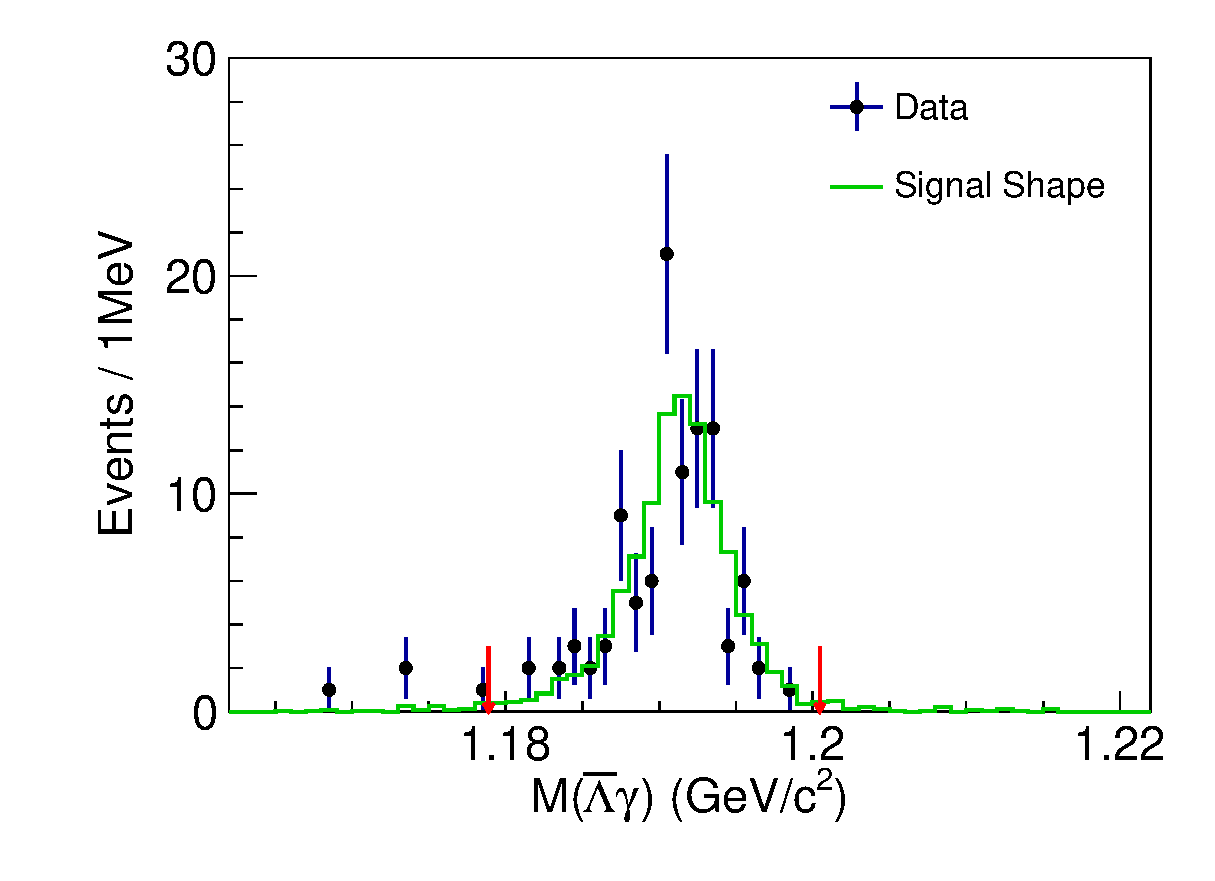
\includegraphics[width=0.8\linewidth]{figures/Sigma/eve/tagmS.eps}
    \caption{$\bar{\Lambda} \gamma$的不变质量谱。
    }%
    \label{fig:tagSigmaMass}
\end{figure}
\section{信号产额}

\subsection{本底分析}%
\label{sec:bkg-ana-sigma0Decay}
本文根据衰变末态的不同将本底分成四类,这四类分别是
\begin{itemize}
        \item 标记$\bar{\Sigma}^{0}$的本底 \\
            由于标记$\bar{\Sigma}^{0}$仅起到压低本底作用,其本底估计不会影响信号
            的产额,从而可以避免考虑这部分的本底估计
        \item 峰本底(比如$J/\psi \to \gamma \Sigma^{0} \bar{\Sigma}^{0}$)\\
            这个本底的特点是包含$\Sigma^{0} \bar{\Sigma}^{0}$对,和信号的末态
            完全重复,故本文把这种过程当成信号看待,只会略微增加信号产额。
        \item 误组合本底 \\
            来源是衰变末态和信号末态完全相同的过程,比如$J/\psi \to \Lambda
            \bar{\Lambda} \pi^{0}(\to \gamma e^{+} e^{-})$。我们首先在include
            蒙特卡洛样本样本中寻找可能的误组合本底,接着从数据中的特征量中观察
            有无可能的潜在本底。
\end{itemize}
本底的定量估计所依赖的遍举过程的分支比取世界测量平均值~\cite{PDG},最主要的几项本底过程
见表~\ref{tab:background}。
\begin{table}[htbp]
    \caption{%
        几种主要的本底。基于蒙特卡洛研究每个本底预期的事例数,每个过程的分支比
        采取世界测量平均值~\cite{PDG}。
    }%
    \label{tab:background}
    \begin{center}
        \begin{tabular} {p{0.6 \linewidth} p{0.2\linewidth}}
            \toprule 
            本底过程  &  预期事例数 \\
            \midrule 
            $J/\psi \to \Lambda \bar{\Sigma}^{*0} +{\rm c.c}$ & $<112$ \\
            $J/\psi \to \Lambda \bar{\Sigma}^{0} + {\rm c.c}$ & 54\\
            $J/\psi \to \gamma \eta_c, \eta_c \to \Lambda \bar{\Lambda}
            $ & 42\\
            $J/\psi \to p \bar{p} \eta, \eta \to \pi^{+} \pi^{-}
            \pi^{0}$ & 17\\

            $J/\psi \to p \bar{p} \pi^{+} \pi^{-} \pi^{0}$ & 13 \\
            $J/\psi \to \Lambda \Lambda \pi^{0}$ & 10 \\
            $J/\psi \to \Sigma^{-} \bar{\Sigma}^{*+} + {\rm c.c}$ & 6 \\

            $J/\psi \to \gamma \eta_c, \eta_c \to \Lambda
            \bar{\Sigma}^{0} + {\rm c.c}$ &  Unknown \\

            $J/\psi \to \gamma  \Lambda
            \bar{\Sigma}^{0} + {\rm c.c}$ &  Unknown \\

            \bottomrule
        \end{tabular}
    \end{center}
\end{table}

一种可能的本底来自$\pi^{0}$介子的达利兹衰变,即$\pi^{0} \to \gamma e^{+}
e^{-}$,为了确认是否有这项本底,我们观察$e^{+}e^{-}\gamma$的不变质量谱,
如图\ref{fig:meeg-sigma0Decay}所示
\begin{figure}[htpb]
    \centering
    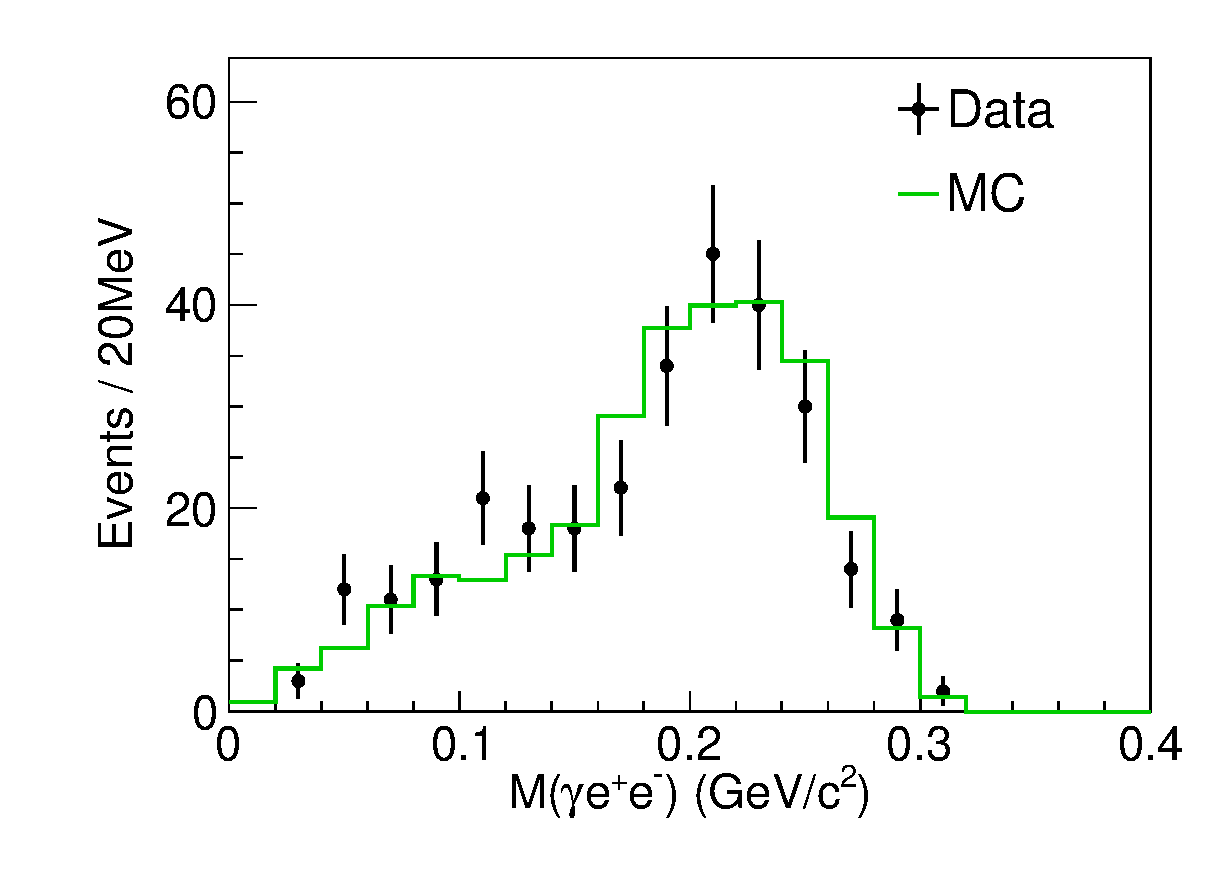
\includegraphics[width=0.8\linewidth]{figures/Sigma/eve/mPi0.eps}
    \caption{%
        $e^{+}e^{-}\gamma$的不变质量谱。
    }%
    \label{fig:meeg-sigma0Decay}
\end{figure}
另一方面,从信号$\Sigma^{0}$的不变质量谱\ref{fig:mSignal}上可以看出几乎没有
任何除$\Sigma^{0} \to \gamma \Lambda$以外的的本底。
\begin{figure}[htpb]
    \centering
    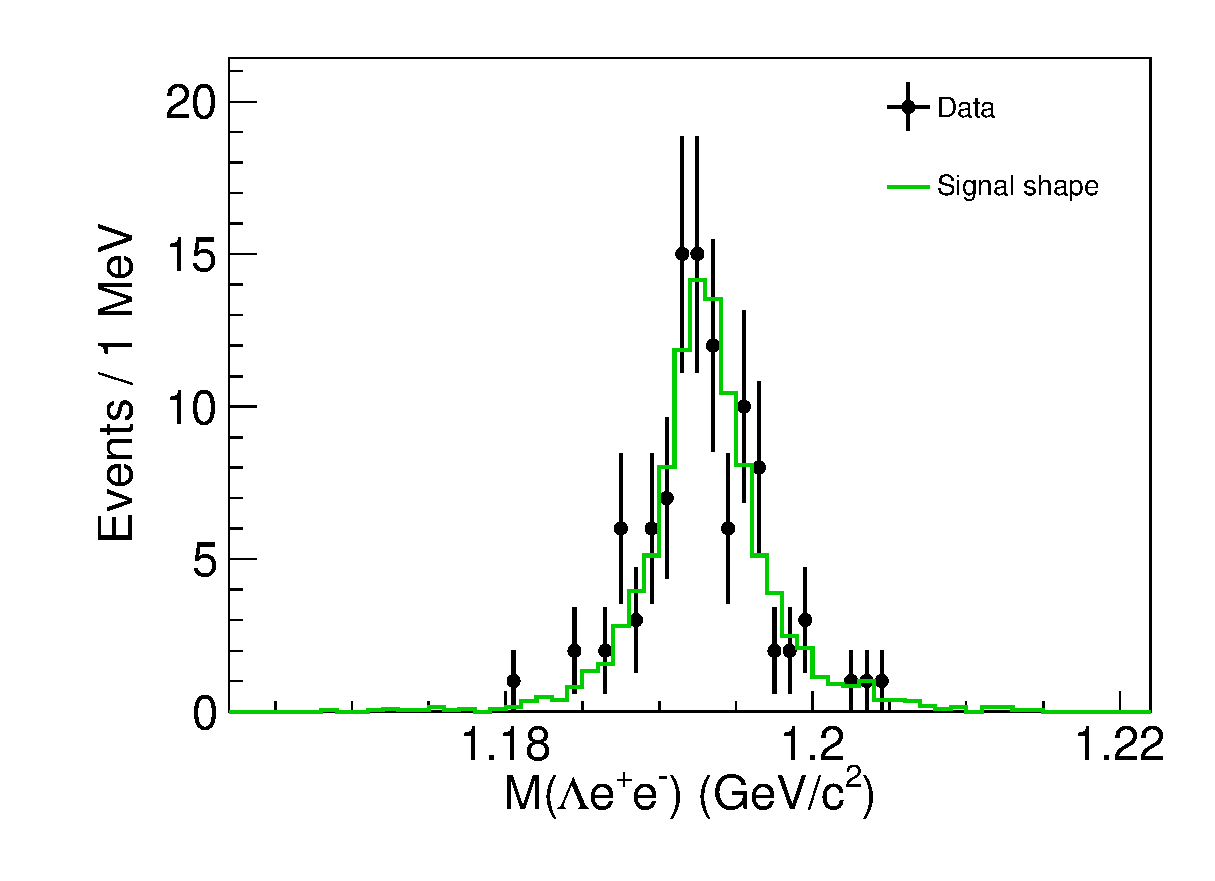
\includegraphics[width=0.8\linewidth]{figures/Sigma/eve/mSignal.eps}
    \caption{$\Lambda e^{+} e^{-}$的不变质量谱。}%
    \label{fig:mSignal}
\end{figure}

\section{寻找$X(17)$粒子}
\begin{figure}[htpb]
    \centering
    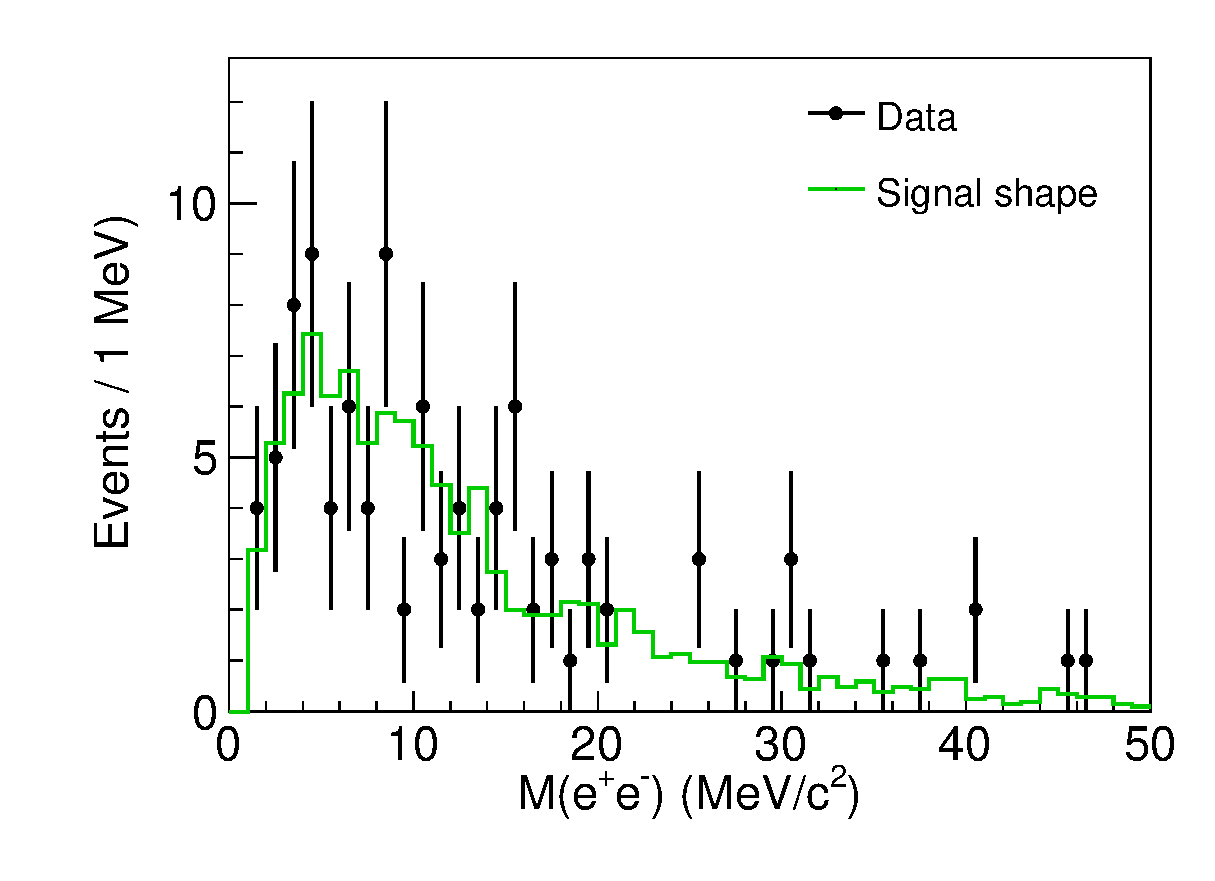
\includegraphics[width=0.8\linewidth]{figures/Sigma/eve/mEE.eps}
    \caption{$e^{+} e^{-}$的不变质量谱。}%
    \label{fig:mEE}
\end{figure}
